画像のレジストレーションの方法に関わらず、画像の変形は画像レジストレーションに必要な要素である。

%画像の変形技術は大別して線形変形および非線形変形の2種類がある。
%本節では画像変形手法について上記の二つの方法を述べる。

\subsection{アフィン変換}
    アフィン変換は幾何平面上で定義される画像に対する最も基本的な変形方法である。
    この変換は、平行移動、拡大縮小、回転、せん断変形を$3\times 3$行列を用いて行われる。
    変換前の座標を$(x,y)$、変形後の座標を$(x^{\prime},y^{\prime})$とすると、アフィン変換は次式で表すことができる。
    \begin{equation}
        \left(\begin{array}{l}
        x^{\prime} \\
        y^{\prime} \\
        1
        \end{array}\right)
        =
        \left(\begin{array}{lll}
        a & b & c\\
        d & e & f\\
        0 & 0 & 1
        \end{array}\right)
        \left(\begin{array}{l}
        x \\
        y \\
        1
        \end{array}\right)
    \end{equation}
    このアフィン変換は、変形によって図形の面積が不変であり、任意のピクセル同士の順序や相対距離が不変である。

    \subsubsection{平行移動}
        アフィン変換において最も基本的な変換は平行移動である。

        \begin{figure}[htbp]
            \begin{minipage}{0.5\hsize}
                \begin{center}
                    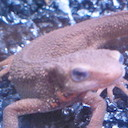
\includegraphics[width=50mm]{./8_appendix/img/imori.jpg}
                \end{center}
                \caption{元画像}
            \end{minipage}
            \begin{minipage}{0.5\hsize}
                \begin{center}
                    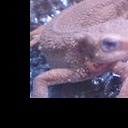
\includegraphics[width=50mm]{./8_appendix/img/imori_Translation.jpg}
                \end{center}
                \caption{x方向に+30、y方向に-30平行移動した後の画像}
            \end{minipage}
        \end{figure}

        平行移動は、x,yそれぞれの移動量を$(d_x, d_y)$とすると、以下の式で定義できる。
        \begin{equation}
            \left(\begin{array}{l}
            x^{\prime} \\
            y^{\prime} \\
            1
            \end{array}\right)
            =
            \left(\begin{array}{lll}
            1 & 0 & d_x\\
            0 & 1 & d_y\\
            0 & 0 & 1
            \end{array}\right)
            \left(\begin{array}{l}
            x \\
            y \\
            1
            \end{array}\right)
        \end{equation}

    \subsubsection{拡大・縮小}
        拡大縮小は、x,yそれぞれの倍率を$S_x, S_y$とすると、以下の式で定義できる。
        \begin{equation}
            \left(\begin{array}{l}
            x^{\prime} \\
            y^{\prime} \\
            1
            \end{array}\right)
            =
            \left(\begin{array}{lll}
            S_x & 0 & 0\\
            0 & S_y & 0\\
            0 & 0 & 1
            \end{array}\right)
            \left(\begin{array}{l}
            x \\
            y \\
            1
            \end{array}\right)
        \end{equation}
        \begin{figure}[htbp]
            \begin{minipage}{0.5\hsize}
                \begin{center}
                    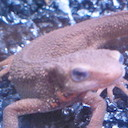
\includegraphics[width=50mm]{./8_appendix/img/imori.jpg}
                \end{center}
                \caption{元画像}
            \end{minipage}
            \begin{minipage}{0.5\hsize}
                \begin{center}
                    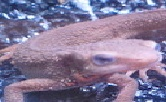
\includegraphics[width=65mm]{./8_appendix/img/imori_Scale.jpg}
                \end{center}
                \caption{x方向に1.3倍、y方向に0.8倍にリサイズした後の画像}
            \end{minipage}
        \end{figure}

        また、このとき$S_x, S_y$を負の値にすることによって、反転処理を実現することができる。
        このような処理を鏡映と呼び、x軸に対して対称の画像を作成する場合には$S_y$を負の値に、y軸に対して対称の画像を作成する場合には$S_x$を負の値にする必要がある。
        このとき、単純に反転を行った場合には画素は画像の範囲から逸脱することに注意する必要がある。
        そのため、計算機上で反転を行う場合には、単純に格納される配列を逆順にする操作を行う場合が多い。

    \subsubsection{回転}
        回転は、角度$\theta$を用いて以下の式で定義できる。
        \begin{equation}
            \left(\begin{array}{l}
            x^{\prime} \\
            y^{\prime} \\
            1
            \end{array}\right)
            =
            \left(\begin{array}{lll}
            \cos{\theta} & -\sin{\theta} & 0\\
            \sin{\theta} & \cos{\theta} & 0\\
            0 & 0 & 1
            \end{array}\right)
            \left(\begin{array}{l}
            x \\
            y \\
            1
            \end{array}\right)
        \end{equation}
        \begin{figure}[htbp]
            \begin{minipage}{0.5\hsize}
                \begin{center}
                    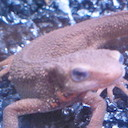
\includegraphics[width=50mm]{./8_appendix/img/imori.jpg}
                \end{center}
                \caption{元画像}
            \end{minipage}
            \begin{minipage}{0.5\hsize}
                \begin{center}
                    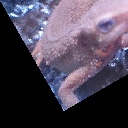
\includegraphics[width=50mm]{./8_appendix/img/imori_Rotate.jpg}
                \end{center}
                \caption{原点を中心として30度回転させた画像}
            \end{minipage}
            \begin{minipage}{0.5\hsize}
                \begin{center}
                    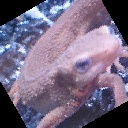
\includegraphics[width=50mm]{./8_appendix/img/imori_Rotate_center.jpg}
                \end{center}
                \caption{画像中心を原点として30度回転させた画像}
            \end{minipage}
        \end{figure}
        また、この場合回転中心は原点、つまり画像の左上になってしまうため、画像中心を原点として回転させる場合には平行移動と上手く組み合わせて利用する必要がある。
    
    \subsubsection{せん断}
        画像を斜め方向に伸ばすような変形をせん断変形と呼ぶ。
        せん断変形は、移動量$(d_x, d_y)$を用いて以下の式で定義できる。
        \begin{equation}
            \left(\begin{array}{l}
            x^{\prime} \\
            y^{\prime} \\
            1
            \end{array}\right)
            =
            \left(\begin{array}{lll}
            1 & \frac{d_x}{h} & 0\\
            0 & 1 & 0\\
            0 & 0 & 1
            \end{array}\right)
            \left(\begin{array}{l}
            x \\
            y \\
            1
            \end{array}\right)
            \label{Xsharing}
        \end{equation}

        \begin{equation}
            \left(\begin{array}{l}
            x^{\prime} \\
            y^{\prime} \\
            1
            \end{array}\right)
            =
            \left(\begin{array}{lll}
            1 & 0 & 0\\
            \frac{d_y}{h} & 1 & 0\\
            0 & 0 & 1
            \end{array}\right)
            \left(\begin{array}{l}
            x \\
            y \\
            1
            \end{array}\right)
            \label{Ysharing}
        \end{equation}
        ここで$h$および$w$は画像の高さおよび幅を表す。

        このとき、式(\ref{Xsharing})のような$x$方向に$d_x$だけ引き伸ばしたような画像はX-sharingと呼ばれ、式(\ref{Ysharing})のような$y$方向に$d_y$だけ引き伸ばしたような画像はY-sharingと呼ばれる。
        \begin{figure}[htbp]
            \begin{minipage}{0.5\hsize}
                \begin{center}
                    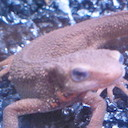
\includegraphics[width=50mm]{./8_appendix/img/imori.jpg}
                \end{center}
                \caption{元画像}
            \end{minipage}
            \begin{minipage}{0.5\hsize}
                \begin{center}
                    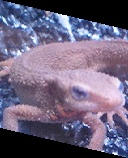
\includegraphics[width=50mm]{./8_appendix/img/imori_xshar.jpg}
                \end{center}
                \caption{x方向に30ピクセルだけ引き伸ばした画像}
            \end{minipage}
            \begin{minipage}{0.5\hsize}
                \begin{center}
                    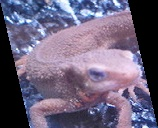
\includegraphics[width=50mm]{./8_appendix/img/imori_yshar.jpg}
                \end{center}
                \caption{y方向に30ピクセルだけ引き伸ばした画像}
            \end{minipage}
        \end{figure}

    \subsubsection{アフィン変換行列の逆行列}
        アフィン変換によって変形した画像を元の画像に戻す際には、アフィン変換行列の逆行列を求める必要がある。
        通常の3次正方元行列と異なり、アフィン変換行列の逆行列は以下のように比較的簡単に求めることができる。
        \begin{align}
            \left(
            \begin{array}{ccc}
                a&b&t_x\\ c&d&t_y\\ 0&0&1 
            \end{array}
            \right)^{-1} 
        &=  \left( 
                \left(
                \begin{array}{ccc}
                    1&0&t_x\\ 0&1&t_y\\ 0&0&1 
                \end{array}
                \right)
                \left(
                \begin{array}{ccc}
                    a&b&0\\ c&d&0\\ 0&0&1
                \end{array}
                \right)
            \right) ^ {-1} \\ 
        &=  \left(
            \begin{array}{ccc}
                a&b&0\\ c&d&0\\ 0&0&1
            \end{array}\right)^{-1}
            \left(
            \begin{array}{ccc}
                1&0&t_x\\ 0&1&t_y\\ 0&0&1
            \end{array}\right)^{-1} \\
        &= \left(
            \begin{array}{ccc}
                d/\Delta{}&-b/\Delta{}&0\\ -c/\Delta{}&a/\Delta{}&0\\ 0&0&1 
            \end{array}
            \right)
            \left(
            \begin{array}{ccc}
                1&0&-t_x\\ 0&1&-t_y\\ 0&0&1
            \end{array}\right)\\
        &= \left(
            \begin{array}{ccc}
            d/\Delta{}&-b/\Delta{}&(-dt_x+bt_y)/\Delta{}\\ -c/\Delta{}&a/\Delta{}&(ct_x-at_y)/\Delta{}\\ 0&0&1
            \end{array}
            \right)
        \end{align}
        

\subsection{射影変換}

\subsection{非線形変形}
    以上のような線形変換では実現できないような複雑な位置合わせを行う場合は非線形変換を行う必要がある.
    \subsubsection{B-spline法}
        非線形位置合わせではB-spline法がよく用いられる.
        ある画素に注目した際に, 近傍4つの制御点から成る変位場とB-spline関数の掛け合わせによって変形が行われる.
        制御点を等間隔$\delta$に設定し, 変位場を$\phi\left(i+m, j+n\right)$とすると, B-spline曲線を用いた非線形変換は以下のように定義される.
        \begin{eqnarray} 
        \mu(x, y)&=&\sum_{m=0}^{3} \sum_{n=0}^{3} B_{m}(u(x)) B_{n}(v(y)) \phi\left(i+m, j+n\right)\\
        i&=&\left|\frac{x}{\delta}\right|-1, j=\left|\frac{y}{\delta}\right|-1\\
        u(x)&=&\frac{x}{\delta}-\left|\frac{x}{\delta}\right|, v(y)=\frac{y}{\delta}-\left|\frac{y}{\delta}\right|\\
        B_{0}(s)=\frac{(1-s)^{3}}{6}, B_{1}(s)&=&\frac{3 S^{3}-6 S^{2}+4}{6}, B_{2}(s)=\frac{-3 S^{3}+3 S^{2}+3 s+1}{6}, B_{3}(s)=\frac{S^{3}}{6}
        \end{eqnarray}
            \begin{figure}[ht]
            \begin{center}
              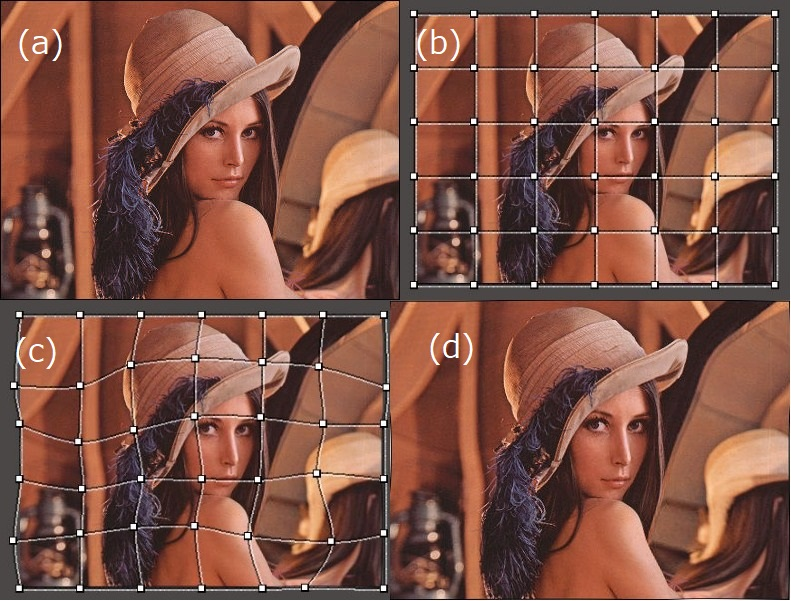
\includegraphics[width=10.0cm]{./8_appendix/img/spline}
            \caption{スプライン曲線を用いた画像変形の例\ (a)元画像\ (b)(c)変形操作\ (d)変形後の画像}
            \label{}
            \end{center}
        \end{figure}

    \subsubsection{Thin-Plate-spline法}

\subsection{Displacement Vector Field}